\chapter{Understanding CUDA}\label{chp:GPGPU}

\chapterquote{Hardware: The parts of a computer system that can be
  kicked.}{Jeff Pesis}



% Motivate the use of GPUs

Because of the evergrowing demand for new effects and more detail in
computer games and other 3D graphics applications, GPU's have seen a
massive increase in computational power over the last decade. This is
evidenced by \reffig{fig:gflops}, which compares the computational
development of NVIDIA GPU's with that of Intel CPU's. A similar figure
comparing the theoretical throughput of GPU's and CPU's can be seen in
\citebook{CUDAPG}. These figures illustrate the potential performance
gain associated with GPU implementations compared to CPU
implementations.

\begin{figure}
  \centering
  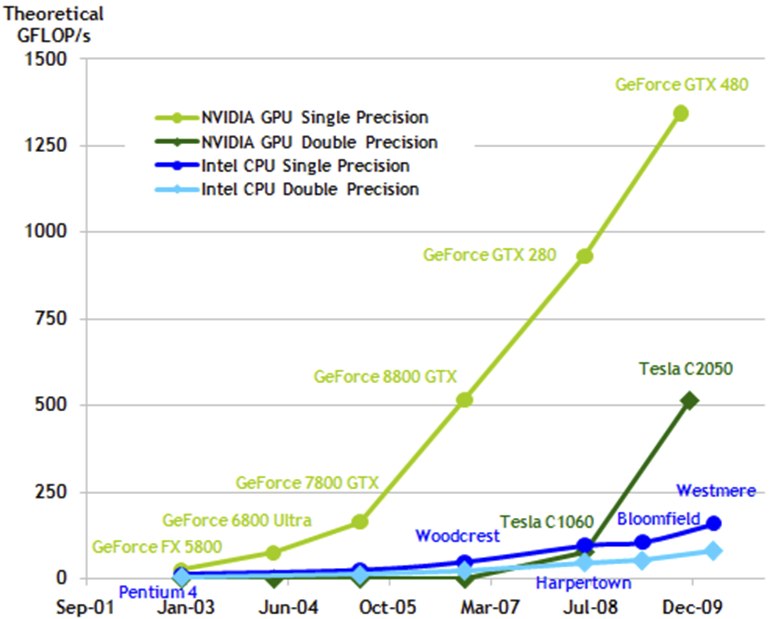
\includegraphics[width=8cm]{GFLOPS}
  
  \parbox{9cm}{\caption[Comparison of floating point operations per
      second on GPU's and CPU's.]{A comparison of the development of
      floating point operations per second on GPU's and CPU's. \\The
      figure is from Chapter 1 in
      \citebook{CUDAPG}.}\label{fig:gflops}}
\end{figure}

% What is different form CPUs

Utilizing all this computational power and throughput effectively,
however, is not straightforward and in order to create algorithms on
the GPU that run faster than their CPU counterparts, we need to
understand how the GPU works.

The reason behind the difference in theoretical throughput seen in
\reffig{fig:gflops}, is that the CPU is designed for handling all
kinds of problems, with a large cache at it's disposal and efficient
handling of control flow. The GPU on the other hand is designed for
high throughput of small, arithmetically intense, \textit{dataparallel
  programs}\footnote{Each instruction is concurrently applied on
  multiple data elements.} called \textit{kernels}, which is exactly
what is required of a graphics card processing thousands of
independent vertices and performing the same color calculations or
\textit{shading} on hundreds of thousands of
\textit{fragments}\footnote{All data needed to generate the color of
  geometry.}.

Since the graphics card is designed to perform vertex and fragment
processing independently of their respective neighbouring threads,
this also means that when programming the graphics card, no
assumptions can be made about which thread is where in it's
execution. This presents a problem in cases where the $n$'th thread
depends on information from all previous $n-1$ threads, e.g. when
splitting data or calculating the minimum or maximum values of $N$
vertices. NVIDIA's CUDA remedies this somewhat by providing
synchronization commands, but since these can only synchronize a
subset of the running threads, the overall problem remains the same.

% Why not use GPU/CPU solutions

An obvious solution is of course to perform easily parallelisable
operations on the graphics card and leave the rest for the
CPU. However, the following quote comes to mind:

\quotebook{
  It is important to include the overhead of transferring data to and
  from the device in determining whether operations should be
  performed on the host or on the device.
}{CUDABPG}

So once it has been decided to use the graphics card, one cannot
simply transfer data back to the CPU for processing and then transfer
it back the GPU. The transfer overhead would in many cases outweigh
the performance increase gained by using the GPU in the first place.

%% Fortunatly Sengupta et al. has come up with a solution to the
%% scattering problem, which will be discussed further in
%% \refsection{sec:GPUprims}.


% Overview of the chapter

Finding effective GPGPU solutions to the above mentioned problems is
the motivation for this chapter, which is structured as follows.
First we shall take a look at how threads and memory are organized in
CUDA. Understanding this will be critical in developing GPGPU
efficient solutions. Then a section will present the GPGPU scan
primitive, which is useful on dataparallel hardware, e.g. when the
address where the result of a threads should be written to is based on
the result of each previous thread, also known as \textit{data
  scattering}. I will then be discussing a couple of interesting
optimization techniques on the GPGPU, while applying them to a case
study.

\section{The Architecture of the GPGPU}

Understand the architecture of CUDA requires us to first
understand the relationship and layout of threads and then the
different kinds of memory available these threads.

CUDA's architecture is based on \textit{multiprocessors}. A
multiprocessor is able to execute hundreds of threads
concurrently. Managing these threads is made easier by a
multiprocessors \textit{SIMT}\footnote{Single-Instruction,
  Multiple-Thread} architecture, in which a single instruction in a
program is relayed to several threads in parallel. A multiprocessor is
equipped with fast, but limited local memory that is used by the
threads currently executing. These multiprocessors enable the graphics
card to handle execution of more than a million threads sequentially.


%% Simply considering a graphics application running at a resolution of
%% 1440x900 where each fragment is shaded should convince anyone of this.

%% While I have above argued that all of these threads are executed
%% independently of each other, NVIDIA's CUDA architecture does place
%% these threads in a hierarchy, which provides programmers with some
%% control over thread execution.

\subsection{The Thread Hierarchy}\label{sec:threadHierarchy}

% Grid, blocks, warps and threads. We will only deal with the one
% dimensional case.

% warps

At the lowest level threads are scheduled and executed completely
parallel in small groups called \textit{warps}\footnote{The term
  originates from weaving, the first parallel thread
  technology.\citebook{CUDAPG}}, usually with a warpsize of 32. A
thread in a warp has its own instruction counter and register state,
and can therefore branch independently of neighbouring
threads. However, a warp can only execute one specific instruction at
a time. The following example should help clarify this.

\begin{algorithmic}
  \IF{threadID < 16}
    \ASSIGN{$x$}{$threadID$}
  \ELSE
    \ASSIGN{$x$}{$32 - threadID$}
  \ENDIF
\end{algorithmic}

% It is a wide SIMD/SIMT, Single-Instruction / Multiple-Thread,
% machine. This means branching hurts. Alot!

The first 16 threads in the warp will evaluate to true and thus
perform the assignment $x \leftarrow threadID$, while the next 16
threads will evaluate to false and execute the alternate statement $x
\leftarrow 32 - threadID$. Since the warp can only perform one
distinct instruction at a time, it will have to first execute $x
\leftarrow threadID$, leaving the last 16 threads idle. It next
executes the else branch, meaning the first 16 threads are now left
idling. While this example shows how branching can hurt performance,
when all threads in a warp do not take the same execution path,
knowning that all threads in a warp are always synchronized can also
be very beneficial, as will be shown in
\refsection{sec:loopUnrolling}.

% TODO explain any/all/ballot?

% blocks

Warps are then organized into 3 dimensional \textit{blocks}. Blocks
are expected to reside on the same multiprocessor, which provides a
limit as to how many threads a block can contain. On current GPU's the
limit can be up to 1024 threads per block or multiprocessor. The size
of blocks is chosen before a kernel is launched and all blocks will
have the same size Having threads executed on the same multiprocessor
comes with a few benefits. It is possible to force synchronized
execution of entire blocks at specific points in the kernels. Threads
can then cooperate through the multiprocessor's fast local memory and
use it to share data. Threads can lookup their \textit{thread index}
inside a block through the 3 dimensional \textit{threadIdx} CUDA
built-in variable. Being able to lookup a threads id is important for
working with data. In the one dimensional case the $n$'th thread will
usually process the $n$'th data element. Without the thread index this
would not be possible.

% grid

Blocks are themselves arranged into the uppermost part of the thread
hierarchy, a 2 dimensional \textit{grid}. The amount of data being
processed usually defines how large the grid will be. Just like a
thread can access it's index or id, it can also lookup it's block
index inside the grid through the built-in \textit{blockDim}. A 2
dimensional thread hierarchy can be seen on
\reffig{fig:threadLayout}. The kernels in this thesis will usually
process the data as 1D linear array, so a threads global id can be
calculated as $id \leftarrow blockDim.x * blockIdx.x + threadIdx.x$.

\begin{figure}
  \centering
  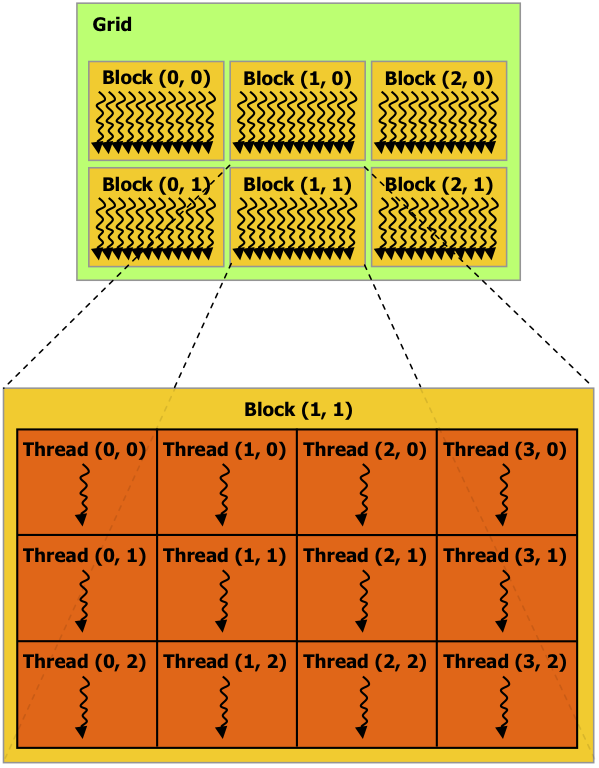
\includegraphics[width=8cm]{ThreadLayout}
  \caption[CUDA's thread hierarchy.]{A figure of CUDA's thread
    hierarchy.\\ The figure is from Chapter 2 in \citebook{CUDAPG}.}
  \label{fig:threadLayout}
\end{figure}




\subsection{The Memory Model}

With the thread hierarchy explained, the different memory spaces made
available through CUDA can be described.  

CUDA provides the programmer with 3 overall types of memory:
\textit{global memory}, which can be accessed by any thread at any
time and persist across kernel launches, \textit{shared memory}, which
is shared across all threads in a block and persists as long as that
block is active, and finally \textit{registers}, which are local to
each thread and only exists as long as it's thread. In the following a
section is devoted to each memory space.

\subsubsection{Global Memory}

% Slow, coalescene of data types with size 1, 2, 4, 8, and 16 bytes.

Global memory, or \textit{device memory}, is the slowest form of
memory on CUDA devices. As mentioned above it persists across kernel
launches and is therefore perfect for storing input data to kernels
and their results. To avoid making lots of memory transactions to and
from global memory, a warp will try to coalesce it's threads' global
memory access into as few transactions as possible. How well
transactions are coalesced depends on the \textit{compute capability}
of the used graphics card, with newer graphics cards being more
flexible. Suffice it to say here that it is preferable to access
global memory sequentially, ie. the $n$'th thread in a warp accesses
the $n$ data element.

% Coalesced memory access, float4 instead of float3
% The alignment requirement can be forced: stuct __align__(8) {

Another restriction on global memory is that data accessed must be of
size 1, 2, 4, 8 or 16 bytes, otherwise memory transactions will be
broken up into multiple requests with an interleaved access pattern
that hinders coallescence. Due to this it is actually more efficient
to use the CUDA built-in struct \textit{float4} than \textit{float3}
when accessing global memory.

For more information on coalescence see Appendix G in
\citebook{CUDAPG}, where the coalescence requirements for hardware of
a specific compute capability is described.

% hiding latency

The scheduler will also help with hiding latency from a global memory
access. If one warp is stalled while waiting for data, another
resident warp that is ready to execute can be scheduled
instead. Utilization of the graphics hardware is therefore heavily
dependent on the number of resident warps and maximizing these can be
important. Especially if memory accesses are scattered, like they will
be when ray tracing a hierarchical structure.

% Mention textures and cache. The project developed for this thesis
% will not be using textures, since global memory also has cache as of
% 2.0 hardware.

\textit{Textures} also reside in device memory space. Textures are
read only 1D, 2D or 3D data arrays, but provide a fast texture cache
optimized for 2 dimensional spatial data locality. This can make
texture access faster than pure global memory access, as a device
memory read is only performed on a cache miss. On current generation
hardware, global memory can use shared memory as a cache, so textures
will not be used in this project.

\subsubsection{Shared Memory}

% Faster than global/local
% Allows threads to share data

Shared memory resides on the multiprocessors and is much faster than
global memory. It is shared by all threads in the same block, which
allows them to share data.

% Used to overcome the limitations of global memory.

A normal usecase for shared memory is local caching of global data
shared across multiple threads. In this case the kernel first loads
data into shared memory, then performs a block-wide synchronization if
necessary and proceeds to operate on the data in shared memory. When
the kernel has finished it's computations, the data is then dumped
back to global memory.

% Can be used as global cache on never CUDA architectures isntead of
% textures and shared mem. nice we laike

As mentioned above, on newer architectures multiprocessor memory can
be used implicitly as a cache for global memory.

% TODO? Bank conflicts, nothing is ever as good as it seems.



\subsubsection{Registers and Local Memory}

% Register

Registers are part of the threads execution context and the fastest
kind of memory on the device. Since there is only a fixed amount of
registers available per multiprocessor, a kernels register usage can
have a high impact on \textit{occupancy}\footnote{The amount of thread
  blocks resident on a multiprocessor, relative to the maximum amount
  possible.}, which in turn can have an impack on the schedulers
ability to hide latency.

% launch bounds

The compiler employs different heuristics to minimize register usage,
while keeping the kernel running efficiently. Sometimes though,
programmers may want to use even fewer registers for specific kernels,
in order to maximize occupancy and global memory latency hiding. To
this end they can aid the compilers heuristics by providing
\textit{launch bounds}. In CUDA 2 arguments can be given as launch
bounds. The first tells the compiler the maximum number of threads per
block that the kernel will ever be invoked with. The second argument
tells the compiler how many blocks should be resident on the
multiprocessor. The compiler can then use this information to derive
upper bounds for the registers available per thread.

% TODO? example



% Local memory

But the compiler cannot always simply reduce the number of registers
to fit inside the launch bounds. If 20 register are needed to hold 20
distinct values, then those values have to be stored somewhere else,
when a programmer demands that only 16 registers be used. In that case
the compiler can use \textit{local memory}, which resides in device
memory and thus has the same high latency and low bandwith as global
memory. Forcing a few registers into local memory to gain occupancy
can be beneficial though, and since all non-idling threads will access
local memory at the same time, there is a high probability that local
memory access can be coalesced.

Kernel variables that the compiler will most likely place in local
memory are:

\begin{itemize}
  \item Any array that from the compilers point of view are
    dynamically indexed.
  \item Structures or arrays that are to large to fit inside registers.
  \item Any variable in the kernel, if the kernel has to many
    variables to place them all in register memory. This is referered
    to as \textit{register spilling}.
\end{itemize}



\section{The Scan Primitive}\label{sec:GPUprims}

% Motivate

As explained above it can be quite hard to perform scattering on
dataparallel hardware. In this section I will outline a solution to
this problem as presented by Sengupta et al\citebook{Sengupta:2007} and
give an example of why this primitive is important when constructing
spatial data structures.

% Prefix sum

The reason for reductions being hard, is that each thread requires
knowledge derived from all threads preceding it. An example taken from
\citebook{Sengupta:2007} is the calculation of a \textit{prefix-sum},
which is a special case of \textit{exclusive scan}. Exclusive scan
takes as input a data array, $[a_0, a_1, a_2, ...]$, and a binary
operator, $\oplus$, with an identity element, $i$. The result of
exclusive scan is then a new array with values $[i, a_0, a_0 \oplus
  a_1, a_0 \oplus a_1 \oplus a_2, ...]$. For prefix-sum the operator
is + and the identity element is 0.

\begin{displaymath}
  \begin{array}{r r r r r r r r r}
    in: & 3 & 1 & 7 & 0 & 4 & 1 & 6 & 3 \\
    out: & 0 & 3 & 4 & 11 & 11 & 14 & 16 & 22 \\
  \end{array}
\end{displaymath}

Calculating the prefix-sum for $n$ elements on the CPU is trivial and
can naïvely be done in $O(n)$ time by iterating over the data array
from start to finish. A naïve implementation in the GPU however would
require each thread to sum up every previous value on it's own,
yielding a time complexity of $O(n^2)$. Instead a dataparallel
algorithm has to be devised that allows threads to cooperatively solve
the problem and doing that as efficiently as the CPU, ie in $O(n)$
time.


% Algorithm

Sengupta et al.\citebook{Sengupta:2007}'s work-efficient prefix-sum
requires two passes over the data, one called \textit{reduce} and
another called \textit{down-sweep}. The algorithm is depicted on
\reffig{fig:segScan}. The figure shows scan being applied to an array
containing 8 elements. Cells with the same colors represent threads
belonging to the same block. The arrows show how data is moved, one
arrow entering a cell represents a copy, while 2 arraws entering
represents the application of $\oplus$ to the data. In the reduce
phase \reffig{fig:segScan} shows how each block's threads are first
responsible for cooperating on reducing their own values. The result
of this reduction is then passed as input to a new reduction kernel,
yielding the final reduced value.

\begin{figure}
  \centering
  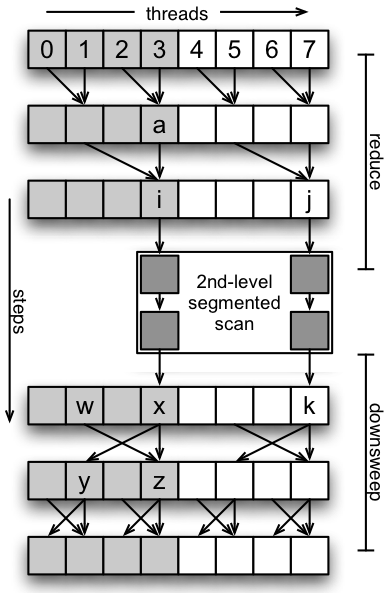
\includegraphics[width=4cm]{SegmentedScan}

  \parbox{5cm}{\caption[Multi-block segmented scan communication.]{An
      example of multi-block segmented scan communication. Cells with
      the same shading belong to the same block. \\The figure is
      borrowed from \citebook{Sengupta:2007}.}\label{fig:segScan}}
\end{figure}

During down-sweep the data is pumped back out into the array, reusing
the reduced values calculated in the previous phase. The result of
this is an array containing the result of a scan application. It can
be quite instructive in dataparallel programming to go through the
algorithm.

For specific details and further implementation optimizations see
Sengupta et al.\citebook{Sengupta:2007}.


% time complexity

For $n$ elements the time complexity of the parallel scan is $2 * O(n
+ n/2 + n/4 + ... + 1) = O(n)$, since the workload is cut in half for
each iteration of the reduce and down-sweep kernels.


% Useful for splitting data

Now the question is: \textit{why is this useful?}. The answer is that
the prefix-sum is vital to splitting data arrays on the GPU. Imagine
an array of triangles that have been split by a splitting plane and
must now be sorted into a new array, with all triangles in front of
the plane sorted to the left and the triangles behind it sorted to the
right. 

\begin{displaymath}
  \begin{array} {r r r r r r r}
    triangles: & [t_0 & t_1 & t_2 & t_3 & t_4 & t_5]\\
    side: & [r & l & r & l & l & r]\\
  \end{array}
  \Rightarrow
  \begin{array} {r r r r r r r}
    &[t_1 & t_3 & t_4 & t_0 & t_2 & t_5]\\
    &[l & l & l & r & r & r]\\
  \end{array}
\end{displaymath}

This needs to be done every time a tree node is split into 2 child
nodes, so being able to do this efficiently on the GPGPU is imperative
to creating kd-trees efficiently.

Obviously the individual threads in a split kernel will have no idea
which address to move the triangle to, since that depends on every
other thread, e.g. $t_0$ must move its data to entry 3, which it can
only do if it knows that it holds the first $r$ and that there are 3
$l$'s. However, by first computing the prefix-sum of the side array,
while adopting the convention that $r = 0$ and $l = 1$, splitting the
triangles become quite easy. Taking the above example the prefix-sum
becomes

\begin{displaymath}
  \begin{array} {r r r r r r r}
    side: & [0 & 1 & 0 & 1 & 1 & 0]\\
    prefix\text{-}sum: & [0 & 0 & 1 & 1 & 2 & 3]
  \end{array}
\end{displaymath}

and the total number of triangles moved left, $nf$, can be found by
adding the last element in $side$ with the last element in $prefix-sum$,
which yields $nf = 0 + 3 = 3$.

The observant reader will have noticed that the prefix-sum actually
calculates the addresses where the triangles on the left side should
be moved to. All that remains is then to calculate the addresses of
the triangles moved right. This is done using $right_i = threadId_i -
prefix_i + nf$.

\begin{displaymath}
  \begin{array} {r r r r r r r}
    right: & [3 & 4 & 4 & 5 & 5 & 5]
  \end{array}
\end{displaymath}

The address that a thread should move it's triangle to is then simply
$address_i = side_i == l$ ? $prefix_i$ : $right_i$ and becomes


\begin{displaymath}
  \begin{array} {r r r r r r r}
    address: & [3 & 0 & 4 & 1 & 2 & 5]
  \end{array}
\end{displaymath}

which will divide the triangles into their respective sides, just like
we wanted.

% TODO? the data keeps it's relation to other elements, which is good
% for coalescence.



\section{Optimization Techniques: Reduction}\label{sec:reduce}

% Motivation: Reduction was important in the previous step and will be
% again for median splitting

In the previous section we saw that it is important to be able to
perform reductions efficiently on the GPU. Calculating the prefix-sum
however isn't the only part of the kd-tree creator where reductions
are needed. It is also useful for calculating the bounding boxes of
the kd-tree's nodes, used when performing median splits.

In this section I will present a naïve \textit{reduction} algorithm
and incrementally apply optimizations to it. A reduction is the
processing of data in some order and building a return value. This
reduction example will use the binary operator \textbf{min}, with
identity element $\infty$, to find the smallest value from it's input
list, but can be generalized to any binary operator with an identity
element. The naïve algorithm is based on the above reduction and will
have an efficient time complexity of $O(n)$, which is the best we can
hope for. Instead of improving the time complexity the following
optimizations will instead focus on making better use of the GPU by
hiding latency, using faster memory where available and reduce the
number of calculations made.

% Works on individual blocks, must be run twice if input is too large
% for one block to handle.

The reduction algorithm will reduce values correctly for individual
blocks. If the input list is too large to be efficiently reduced by
one block, then the algorithm can be run recursively on it's own
output, until a single result is found.

The algorithm assumes that the length of the input list is a power of
2. If that is not the case then either the data could be preprocessed
or the kernel itself can pad the data with the binary operators
identity element.

\subsection{Naïve implementation}

The naïve algorithm, presented in \refalg{alg:naiveReduct}, is a
straight forward implementation of the interleaved access pattern
shown in \reffig{fig:segScan}. The algorithm uses the modulo operator
to distinguish which threads are done and which should continue to
perform reductions. All intermittent values are written back into
global memory, to allow other threads to access the reduced values
when needed. When the block has finished the reduction, the result
is returned by the first thread.

\begin{algorithm}
  \caption{Naïve reduction}
  \label{alg:naiveReduct}
  \begin{algorithmic}
    \PROCEDURE{Reduce0}
              {$values$ : Number List; $id$ : Integer; $elements$ : Integer}
              {$result$ : Number}
              {\ASSIGN{$offset$}{$1$}
                \WHILE{$offset < elements$}
                  \IF{$id$ \MOD  $offset = 0$}
                  \ASSIGN{$values[id]$}{\MIN{$values[id]$}{$values[id + offset]$}}
                  \ENDIF
                  \ASSIGN{$offset$}{$offset * 2$}
                  \SYNC
                \ENDWHILE
                \IF{$id = 0$}
                  \ASSIGN{$result$}{$values[0]$}
                \ENDIF
              }
  \end{algorithmic}
\end{algorithm}

\subsection{Coalesced Memory Access}

Of course there are several inefficiencies to correct in
\refalg{alg:naiveReduct}. To start with we will focus on global memory
access and update it to allow the warp to perform memory accesses
coalesced. Since we're interested in a global reduction it won't
matter in which order values are compared. This allows the interleaved
access pattern to be exchanged with a sequential one, which will
allow the warp to perform coalesced memory access.

%% Also better warp utilization as most threads are active and we get
%% rid of the slow mod operator.

Two pleasent side effects of this change, as shown in
\refalg{alg:coalescedReduct} is that the slow modulo operator has
disappeared and warp utilization has dramatically increased, since the
first $offset$ threads in a block are now live, compared to every
$offset$'th thread in the previous implementation.

\begin{algorithm}
  \caption{Coalesced reduction}
  \label{alg:coalescedReduct}
  \begin{algorithmic}
    \PROCEDURE{Reduce1}
              {$values$ : Number List; $id$ : Integer; $elements$ : Integer}
              {$result$ : Number}
              {\ASSIGN{$offset$}{$elements / 2$}
                \WHILE{$offset > 1$}
                  \IF{$id < offset$}
                  \ASSIGN{$values[id]$}{\MIN{$values[id]$}{$values[id + offset]$}}
                  \ENDIF
                  \ASSIGN{$offset$}{$offset / 2$}
                  \SYNC
                \ENDWHILE
                \IF{$id = 0$}
                  \ASSIGN{$result$}{$values[0]$}
                \ENDIF
              }
  \end{algorithmic}
\end{algorithm}

% TODO? Figure of sequential access


\subsection{Working from Shared Memory}

Even with coalesced memory acces, continuosly accessing global memory
is still quite slow. To remedy this the implementation in
\refalg{alg:sharedReduct} first copies the data into shared memory
before performing any reductions. As can be seen the threads are
working together to perform the copy. Instead of all threads having to
copy the entire data, each thread only fills the $id$'th cell in the
shared list and leaves the other cells to be filled by the other
threads. The subsequent synchronization ensures that all the data has
been copied before proceding with the reduction. Since the threads are
still accessing data sequentially, this change preserves coalescence.

\begin{algorithm}
  \caption{Shared memory reduction}
  \label{alg:sharedReduct}
  \begin{algorithmic}
    \PROCEDURE{Reduce2}
              {$values$ : Number List; $id$ : Integer; $elements$ : Integer}
              {$result$ : Number}
              {\DECLARE{$sValues$}{\textbf{shared} Number List}
                \ASSIGN{$sValues[id]$}{$values[id]$}
                \SYNC
                \ASSIGN{$offset$}{$elements / 2$}
                \WHILE{$offset > 1$}
                  \IF{$id < offset$}
                  \ASSIGN{$sValues[id]$}{\MIN{$sValues[id]$}{$sValues[id + offset]$}}
                  \ENDIF
                  \ASSIGN{$offset$}{$offset / 2$}
                  \SYNC
                \ENDWHILE
                \IF{$id = 0$}
                  \ASSIGN{$result$}{$sValues[0]$}
                \ENDIF
              }
  \end{algorithmic}
\end{algorithm}

\subsection{Using Registers}

Shared memory is quite fast, but registers are even faster. Inspecting
the statement \MIN{$sValues[id]$}{$sValues[id + offset]$}, we can see
that the $id$'th thread will always acces the value stored in
$sValues[id]$ and is the only thread writting to that cell. This
provides us with the possibility to use a register to store this value
in instead. We just have to remember to also store the reduced value
in shared memory, in case another thread needs to use it in the next
iteration. The resulting changes can be seen in
\refalg{alg:registerReduct}.

\begin{algorithm}
  \caption{Register reduction}
  \label{alg:registerReduct}
  \begin{algorithmic}
    \PROCEDURE{Reduce3}
              {$values$ : Number List; $id$ : Integer; $elements$ : Integer}
              {$result$ : Number}
              {\DECLARE{$sValues$}{\textbf{shared} Number List}
                \ASSIGN{$rValue \leftarrow sValues[id]$}{$values[id]$}
                \SYNC
                \ASSIGN{$offset$}{$elements / 2$}
                \WHILE{$offset > 1$}
                  \IF{$id < offset$}
                  \ASSIGN{$rValue \leftarrow sValues[id]$}{\MIN{$rValue$}{$sValues[id + offset]$}}
                  \ENDIF
                  \ASSIGN{$offset$}{$offset / 2$}
                  \SYNC
                \ENDWHILE
                \IF{$id = 0$}
                  \ASSIGN{$result$}{$rValue$}
                \ENDIF
              }
  \end{algorithmic}
\end{algorithm}



\subsection{Loop unrolling}\label{sec:loopUnrolling}

% Unroll the loops: Only works if the number of reductions are known
% beforehand (or if we pad the input)

The final optimization that we will apply to the reduction algorithm
is loop unrolling. As stated above we assume that we know beforehand
how many elements will need to be reduced by the blocks. We now extend
this assumption with the condition that all blocks reduce the same
number of elements. Again this can be accomplished quite easily by
padding the input values when copying them to shared memory. There are
several reason as to why loop unrolling can increase
performance. Firstly looping requires indirection and even though most
of the threads in our warps will loop the same amount of times, the
warps still incur an overhead by having to perform the
indirection. Secondly unrolling removes the overhead of updating the
$offset$ variable, which is a quite significant portion of the work
performed by the kernel when the body inside the loop is this
small. Thirdly we can take advantage of warp synchronization and
remove explicit synchronization invocations when offset becomes less
than the warpsize.

% Then move the first up to where data is loaded into shared mem. And
% move the last reduction down where the final result is written.

After having unrolled the loop, it is now also possible to move thread
0's last reduction, \MIN{$rValue$}{$sValues[1]$}, down to where the
result is output. We are also able to inline the first reduction where
the data is copied from global memory to shared memory, reducing the
shared memory requirements by half per
block. \refalg{alg:unrollReduct} shows the inlining of the first and
final reduction. Unrolling the loop is quite straightforward, but
takes a lot of space and have therefore been omitted here.

% Left as an exercise to the reader :)

\begin{algorithm}
  \caption{Unrolling reduction loops}
  \label{alg:unrollReduct}
  \begin{algorithmic}
    \PROCEDURE{Reduce4}
              {$values$ : Number List; $id$ : Integer; $elements$ : Integer}
              {$result$ : Number}
              {\ASSIGN{$offset$}{$elements / 2$}
                \DECLARE{$sValues$}{\textbf{shared} Number List}
                \ASSIGN{$rValue \leftarrow sValues[id]$}{\MIN{$values[id]$}{$values[id + offset]$}}
                \SYNC
                \ASSIGN{$offset$}{$offset / 2$}
                \WHILE{$offset > 2$}
                  \IF{$id < offset$}
                  \ASSIGN{$rValue \leftarrow sValues[id]$}{\MIN{$rValue$}{$sValues[id + offset]$}}
                  \ENDIF
                  \ASSIGN{$offset$}{$offset / 2$}
                  \SYNC
                \ENDWHILE
                \IF{$id = 0$}
                  \ASSIGN{$result$}{\MIN{$rValue$}{$sValues[1]$}}
                \ENDIF
              }
  \end{algorithmic}
\end{algorithm}
